%%==================================================================%%
%% Author : Abascal Fern�ndez, Patricia                             %%
%% Author : S�nchez Barreiro, Pablo                                 %%
%% Version: 1.1, 21/04/2013                                         %%
%%                                                                  %%
%% Memoria del Proyecto Fin de Carrera                              %%
%% Cap�tulo Domain Engineering, Archivo ra�z                        %%
%%==================================================================%%

\chapterheader{Ingenier�a del Dominio}{Ingenier�a del Dominio}
\label{chap:domain}

En este cap�tulo se describe la fase de \emph{Ingenier�a del Dominio} (en ingl�s, \emph{Domain Engineering}) de nuestra l�nea de productos software. Dentro de dicha fase .....................

\chaptertoc

\section{Transformaciones de Modelo UML a C\#}
\label{domain:sec:transf}

%%%==================================================================%%
%% Author : Abascal Fern�ndez, Patricia                             %%
%% Author : S�nchez Barreiro, Pablo                                 %%
%% Version: 1.2, 21/04/2013                                         %%
%%                                                                  %%
%% Memoria del Proyecto Fin de Carrera                              %%
%% Domain Engineering/Transformaci�n UML a C#                       %%
%%==================================================================%%
\begin{table}%
\begin{tabularx}{15cm}{|l|X|}
\hline
{\bf Elemento en UML} & {\bf Elemento en C\#} \\
\hline
   % Modelo
\multicolumn{ 1}{|l|}{Modelo} &
   Namespace del proyecto. Los namespaces permiten agrupar entidades tales como paquetes, clases, objetos y funciones bajo el mismo nombre. De esta forma, se pueden tener varios namespaces en el mismo proyecto que son independientes entre s�. \\
\hline
   % Paquete
\multicolumn{ 1}{|l|}{Paquete �} &
    Puede ser un directorio, con el mismo nombre que dicho paquete en el modelo, y que contenga tantos ficheros como clases o interfaces almacene en su interior. O un directorio vac�o, con el mismo nombre que dicho paquete en el modelo, por cada paquete vac�o que haya en el modelo UML.   \\
\hline
   % Atributo
\multicolumn{ 1}{|l|}{Atributo} &
    Cada atributo ser� tratado como una propiedad de C\# con los correspondientes m�todos getter y setter. Si el atributo tiene visibilidad \emph{protected} o es \emph{static} no poseer� los m�todos getter y setter. \\
\hline
   % Par�metro
\multicolumn{ 1}{|l|}{Par�metro} &
    Despu�s de identificar si es de retorno de una operaci�n o de entrada a la misma se aplica la transformaci�n al tipo de dato correspondiente.\\
\hline
    % Clase
\multicolumn{ 1}{|l|}{Clase} &
    Clase parcial C\# siguiendo el patr�n slicer, es decir $<$nombre del paquete al que pertenece$>$\_$<$nombre de la clase$>$. Al crear la clase, a�adir tambi�n los m�todos de utilidad. \\
\hline
   % Interfaz
\multicolumn{ 1}{|l|}{Interfaz} &
   Interfaz C\#  implementada siguiendo el patr�n slicer. \\
\hline
   % Operacion
\multicolumn{ 1}{|l|}{Operaci�n} &
    M�todo C\# privado y renombrado siguiendo el patr�n slicer de la forma $<$nombre del paquete al que pertenece$>$\_$<$nombre de la operaci�n$>$, para evitar posibles conflictos, todos los m�todos ser�n virtuales. Los m�todos \emph{protected} no se cambiar�n a privados para respetar la visibilidad requerida inicialmente por el usuario.  \\
\hline
   % Constructor
\multicolumn{ 1}{|l|}{Constructor} &
    Cada clase parcial correspondiente a una caracter�stica tendr� un m�todo privado llamado $<$nombre del paquete al que pertenece$>$\_init$<$nombre de la clase$>$ que contendr� la porci�n de constructor que corresponde a la caracter�stica. \\
\hline
   % Asociaci�n entre clases
\multicolumn{ 1}{|l|}{Asociaci�n} &
    \emph{Asociaci�n simple:} Se a�ade el atributo, simple o colecci�n, de tipo Class a la clase destino.\\
\multicolumn{ 1}{|l|}{} &
    \emph{Asociaci�n bidireccional:} Dependiendo del tipo de bidireccionalidad (one to one, one to many o many to many) se a�aden los atributos y m�todos adicionales necesarios para implementar el correcto funcionamiento de dicha asociaci�n.  \\
\hline
   % Generalizaci�n
\multicolumn{ 1}{|l|}{Generalizaci�n} &
    \emph{Herencia simple:} Una clase hereda de otra clase.\\
\multicolumn{ 1}{|l|}{} &
    \emph{Herencia m�ltiple:} Una clase hereda de varias clases y se debe realizar la transformaci�n correspondiente mediante la creaci�n de interfaces ya que en C\# no se permite la herencia m�ltiple de varias clases pero s� de varias interfaces.   \\
\hline
\end{tabularx}
  \caption{Transformaci�n de elementos del modelo UML a c�digo C\#}
  \label{dom:fig:tranf}
\end{table}%

 \begin{figure}[!tb]
  \centering
  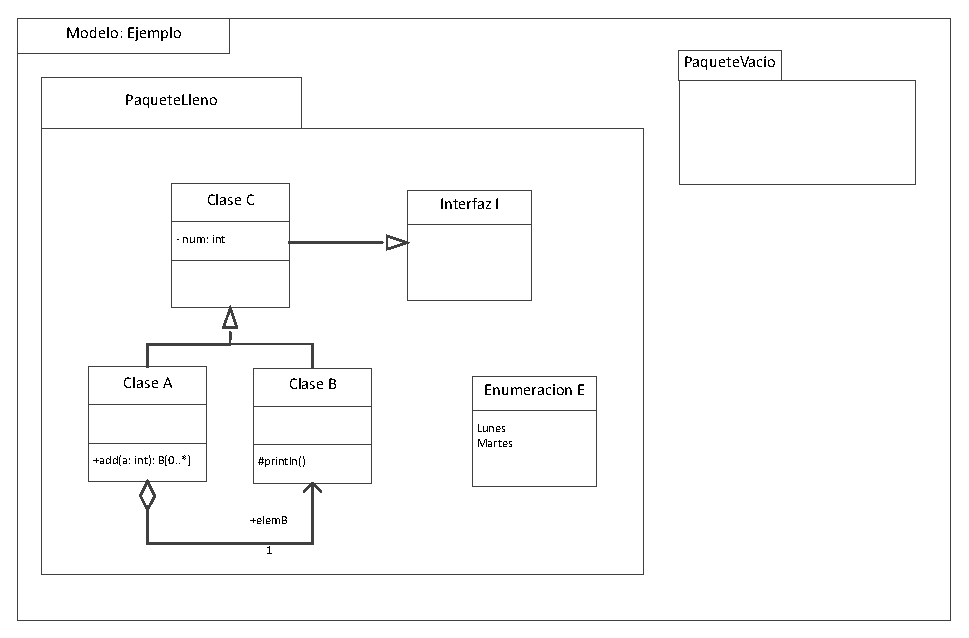
\includegraphics[width=.95\linewidth]{domainEngineering/images/Transformaciones.eps} \\
  \caption{Ejemplo de Modelo UML simplificado}
  \label{dom:fig:ejemplo}
\end{figure}

 El primer paso para la transformaci�n de modelo a c�digo (\emph{model-to-text}, M2T) es la identificaci�n de los distintos elementos que nos podemos encontrar en un diagrama de clases UML y hallar el equivalente en c�digo (C\# en nuestro caso). Hay que tener en cuenta que la transformaci�n no es trivial y es necesario procesar la informaci�n obtenida del modelo para generar el c�digo adecuadamente. En la tabla \ref{dom:fig:tranf} se encuentra un resumen de dicho proceso. A continuaci�n se procede al an�lisis m�s detallado de cada uno de los elementos de dicha tabla, para ello nos apoyaremos en la figura \ref{dom:fig:ejemplo}.
\begin{figure}[tb!]
\begin{center}
\begin{footnotesize}
\begin{verbatim}
File PaqueteLleno/B.cs
--------------------------------------------------------
01 namespace Ejemplo{
02     partial class B: C{
03          ...
04          private virtual void B_initB ( ) {}
05          protected virtual PaqueteLleno_println ( ) {}
06     }
07 }

File PaqueteLleno/A.cs
--------------------------------------------------------
08 namespace Ejemplo{
09     partial class A: C{
10          private B elemB;
11          public B elemB {
12              get { return this.elemB; }
13              set { this.elemB= value; }
14          }
15          ...
16          private virtual void A_initA ( ) {}
17          private virtual ISet<B> PaqueteLleno_add (int a) { }
18     }
19 }

File PaqueteLleno/C.cs
--------------------------------------------------------
20 namespace Ejemplo{
21      partial class C: I{
22          private int num;
23          public int num {
24              get { return this.num; }
25              set { this.num= value; }
26          }
27          ...
28          private virtual void C_initC ( ) {}
29      }
30 }

File PaqueteLleno/I.cs
--------------------------------------------------------
31 namespace Ejemplo{
32     partial interface I{			
33          public virtual override bool Equals (Object o);
34          public virtual override int CompareTo (Object o);
35          public virtual override int GetHashCode ( );
36          public virtual override Type GetType ( );
37          public virtual override string ToString( );
38          private virtual void I_initI ( ) {}
39     }
40 }
\end{verbatim}
\end{footnotesize}
\end{center}
\caption{C�digo generado para las clases y la interfaz del modelo de la figura \ref{dom:fig:ejemplo}}
\label{dom:code:ejemplo}
\end{figure}

El modelo de la figura \ref{dom:fig:ejemplo} es \imp{Ejemplo} y por tanto cada clase del proyecto deber�a comenzar definiendo el namespace del modelo en cuesti�n mediante la l�nea de c�digo C\# tal como se aprecia en las l�neas 1, 8, 20 y 31 de la figura \ref{dom:code:ejemplo}.

En la figura \ref{dom:fig:ejemplo} hay dos paquetes \imp{PaqueteLleno} y \imp{PaqueteVac�o}, por tanto, en el directorio destino donde se generan los ficheros del modelo deber�n aparecer dos carpetas con dichos nombres. La carpeta \imp{PaqueteLleno} contendr� en su interior cuatro ficheros denominados A.cs, B.cs, C.cs e I.cs (jerarqu�a indicada en las l�neas 1, 11, 26 y 40 de la figura \ref{dom:code:ejemplo}), uno por cada clase o interfaz que se encuentra en su interior, mientras que la carpeta \imp{PaqueteVac�o} no contendr� ning�n archivo en su interior.

Tal como se aprecia en la figura \ref{dom:fig:ejemplo}, la clase \imp{A} del paquete \imp{PaqueteLleno}, tiene un atributo llamado \imp{num} por lo que se genera una propiedad con sus respectivos m�todos getter y setter tal como se muestra en la figura \ref{dom:code:ejemplo} en las l�neas 22-26.

La figura \ref{dom:fig:ejemplo} presenta la clase \imp A con una operaci�n \imp{add} que tiene un par�metro \imp{a: int} y retorna una colecci�n de elementos de tipo \imp{B} (figura \ref{dom:code:ejemplo} l�nea 17). De la misma forma, la clase \imp{B} tiene una operaci�n \imp{println} de car�cter \emph{protected} y por tanto su visibilidad no se transforma en \emph{private} (figura \ref{dom:code:ejemplo} l�nea 5). Con este ejemplo quedan ilustrados los puntos de operaci�n y par�metro descritos en la tabla \ref{dom:fig:tranf}.

Para la generaci�n de clases e interfaces de la figura \ref{dom:fig:ejemplo}, el resultado ser�a el mostrado en las l�neas 2, 9, 21 y 32 de la figura \ref{dom:code:ejemplo}. Se aprecia tambi�n las herencias correspondientes.

Aunque no est� reflejado en el modelo UML a�adimos a cada clase, o interfaz, del modelo a�adimos un constructor (figura \ref{dom:code:ejemplo} l�neas 4, 16, 28 y 38) y unos m�todos de utilidad (figura \ref{dom:code:ejemplo} l�neas 33-37).

Por �ltimo, la asociaci�n simple de las clases \imp{A} y \imp{B} se traduce con las l�neas de c�digo descritas en las l�neas 10-14 de la figura \ref{dom:code:ejemplo}.

Con esto queda explicado m�s detalladamente la transformaci�n de modelo UML a c�digo C\# descrita en la tabla \ref{dom:fig:tranf}. Se han omitido la herencia m�ltiple y las asociaciones bidireccionales por su complejidad. En la siguiente secci�n se profundizar� en la implementaci�n y creaci�n de las transformaciones de modelo UML a c�digo C\#.


\section{Generadores de C�digo C\#}
\label{domain:sec:transf}

%%%==================================================================%%
%% Author : Abascal Fern�ndez, Patricia                             %%
%% Author : S�nchez Barreiro, Pablo                                 %%
%% Version: 2.9, 25/04/2013                                         %%
%%                                                                  %%
%% Memoria del Proyecto Fin de Carrera                              %%
%% Domain Engineering/Generadores de C�digo C#                      %%
%%==================================================================%%

Para implementar los generadores de c�digo, se procedi� en encapsular cada una de las reglas descritas en la secci�n anterior en un \emph{template} de EGL. Adem�s, se crearon una serie de funciones auxiliares en EOL. Por ejemplo, se cre� una funci�n auxiliar para determinar el tipo de colecci�n que debe ser utilizada para transformar un atributo multivaluado, es decir, con cota superior de su multiplicidad mayor que uno.

Uno de los mayores problemas que normalmente plantean los generadores de c�digo es que la generaci�n de c�digo es secuencial, no permitiendo la vuelta a atr�s. Por ejemplo, si generamos una clase y m�s tarde descubrimos que dicha clase debe ser modificada porque act�a como clase padre en una herencia m�ltiple, ya no podremos volver a abrir dicha clase para a�adirle la relaci�n de herencia con la interfaz que ha de crearse.

Por tanto, antes de generar una clase, debemos asegurarnos de que no va a necesitar ser modificada posteriormente. Ello implica que hay que tener especial cuidado a la hora de dise�ar el orden en el cual se ejecutan las plantillas, o \emph{templates} de generaci�n de c�digo. La Figura~\ref{dom:fig:templates} muestra el orden de ejecuci�n de las plantillas creadas en nuestro caso. Explicamos parte de dicha figura, aunque no la describiremos entera, por razones de espacio.

\begin{figure}[!tb]
  \center
  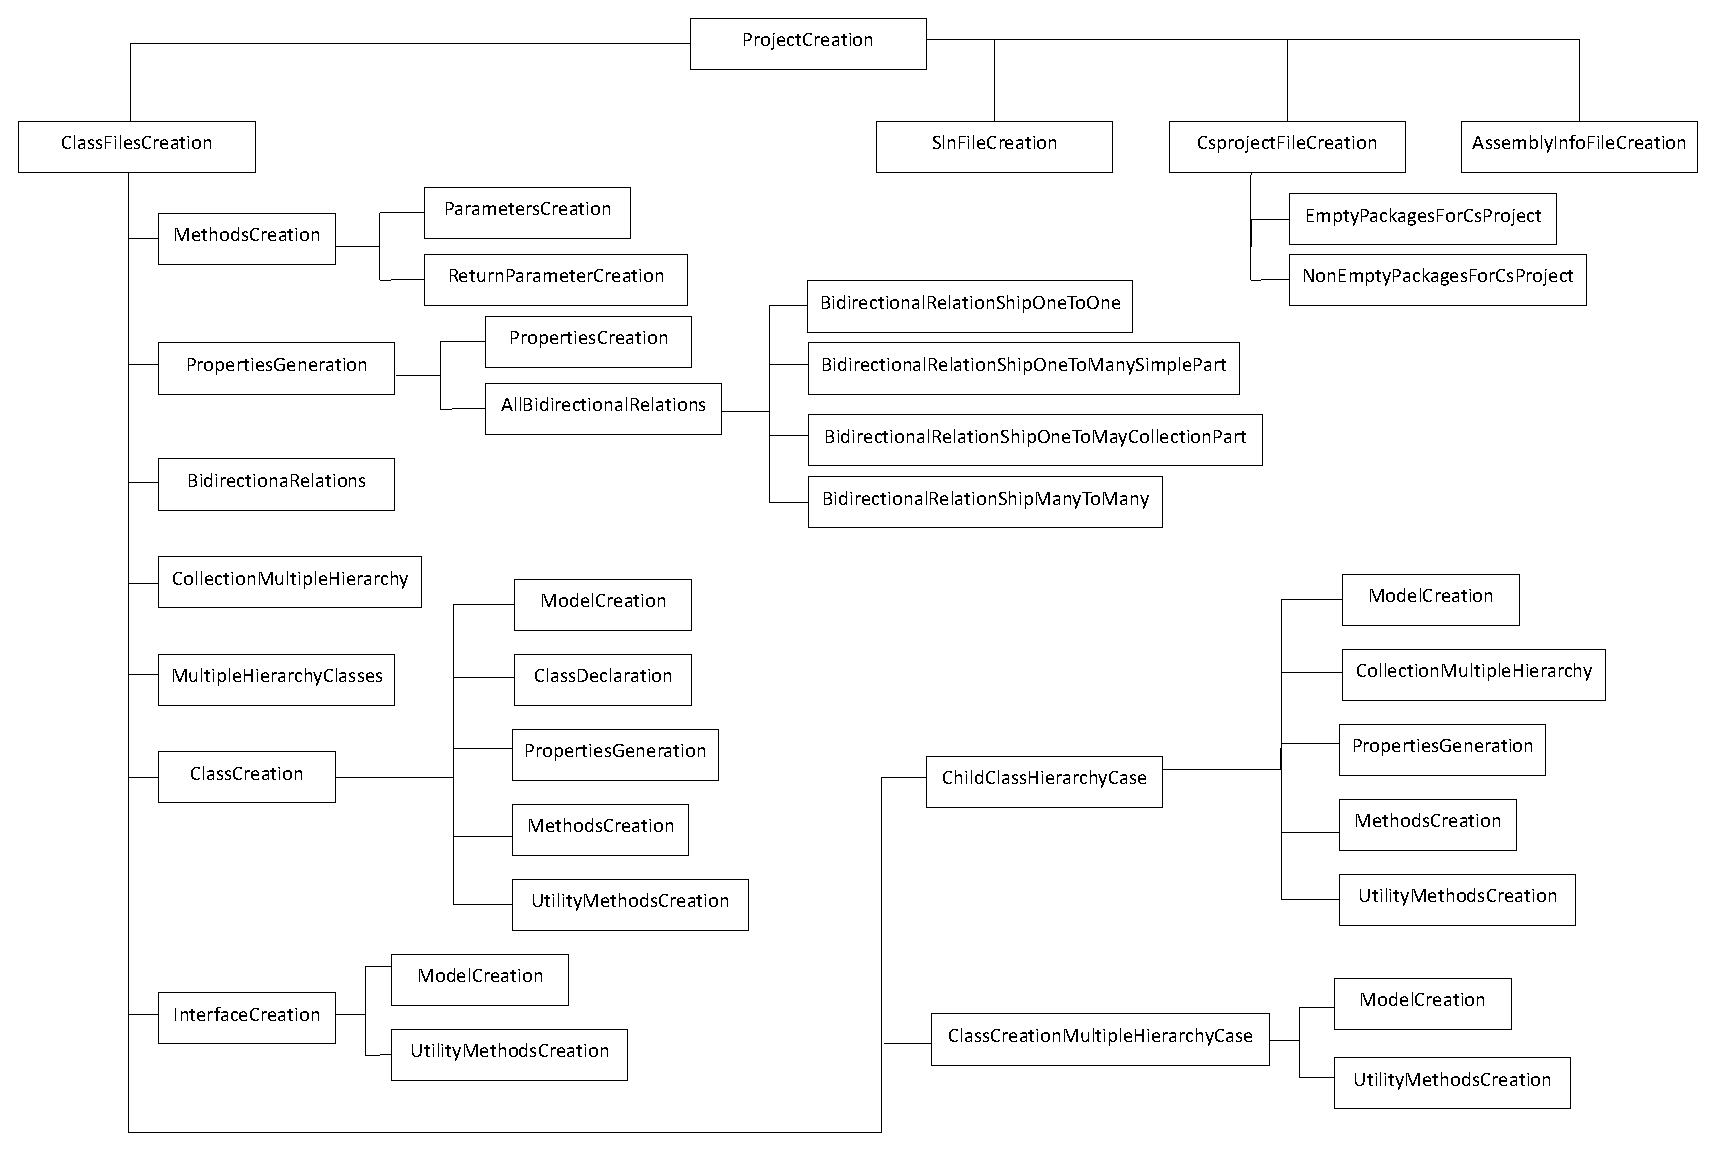
\includegraphics[width=\linewidth]{domainEngineering/images/Templates.eps} \\
  \caption{Orden de ejecuci�n de las plantillas de generaci�n de c�digo}
  \label{dom:fig:templates}
\end{figure}

El punto de partida es el generador de c�digo llamado \imp{ProjectCreation}, encargado de procesar el elemento \emph{modelo}, que constituye la ra�z del proyecto, as� como los \emph{paquetes} que contiene dicho modelo, adem�s de crear el proyecto \emph{Visual Studio 2010} que constituye la salida del generador.  Dicho \emph{template} tiene , por tanto, dos tareas claramente diferenciadas: (1) por una parte, debe generar el c�digo correspondiente a la arquitectura de referencia, lo que se hace a trav�s de la plantilla \imp{ClassFilesCreation}; y (2) por otra parte, debe generar todos los ficheros auxiliares y la estructura que constituyen un proyecto \emph{Visual Studio 2010}, como el fichero de construcci�n (fichero \emph{.csproj}) que indica que clases parciales deben compilarse cuando se construye el proyecto (ver Figura~\ref{back:code:partialClasses}). Para generar estos ficheros auxiliares, se utilizan las plantillas \imp{SlnFileCreation},  \imp{CsprojectFileCreation} y \imp{AssemblyInfoFileCreation}.

La plantilla \imp{ProcessPackageContents} procesa por cada paquete, su contenido. Dependiendo del tipo de cada elemento, se realiza una acci�n diferente, tal como se describe a continuaci�n.

Si se trata de una clase enumerada, se invoca el template \imp{EnumerationClassCreation}, con dicho elemento como argumento.

Se procesan todas las clases con herencia m�ltiple, para aplicar el \emph{mixin pattern}. Para ello se ejecutan las plantillas \imp{ParentImplMultipleInheritanceCase}, que se encarga de procesar las clases padre involucradas en herencias m�ltiples; y \imp{ParentInterfaceMultipleInheritanceCase}, que se encarga de crear las interfaces para estas clases padre. Ambas plantillas hacen uso de las plantillas \imp{MethodsCreation} y \imp{UtilityMethodsCreation}, encargadas de procesar los m�todos de dichas clases e interfaces y de crear los m�todos de infraestructura que fuesen necesarios, tal como \imp{Equals} o \imp{CompareTo}.

A continuaci�n, se ejecuta la plantilla \imp{ChildClassMultipleInheritance}, encargada de procesar una clase hija involucrada en herencia m�ltiple. Para ello se procesan el esqueleto de la clase \imp{ClassDeclaration}, sus atributos (\imp{PropertiesGeneration}), sus m�todos \imp{MethodsCreation} y sus m�todos de infraestructura \imp{UtilityMethodsCreation}.

Seguidamente, se procesan las clases no afectadas, como hijas o como padres, por herencia m�ltiple. Estas clases se procesan a trav�s de la plantilla \imp{ClassCreation}, que funciona igual que la plantilla \imp{ChildClassMultipleInheritance}, a excepci�n de que no se genera el c�digo de los delegados para los \emph{mixins}.

Cada plantilla invocada hace uso a su vez de otras subplantillas, que por razones de claridad y espacio no detallamos. Por ejemplo, la plantilla \imp{PropertiesGeneration} encargada de procesar atributos y extremos de asociaci�n, hace uso de diversas plantillas para procesar los extremos pertenecientes a asociaciones doblemente navegables, tal como se indica en la Figura~\ref{}.

Por �ltimo, comentar que todas las plantillas utilizan diversas funciones auxiliares especificadas en EOL. Por ejemplo, existen funciones para determinar si una clase est� involucrada en una herencia m�ltiple o para devolver todas las clases padre de una clase dada. Adem�s, junto con las funciones auxiliares de EOL, se han creado una serie de funciones auxiliares en Java, invocables desde EOL, y EGL, lo que se conoce en argot Epsilon como una \emph{Java Tool}, para poder manipular el sistema de ficheros. Esto era necesario, por ejemplo, para poder crear la estructura de carpetas del proyecto Visual Studio 2010.

Adem�s, se crearon algunas \emph{Java Tool} para poder mostrar cuadros de di�logo que permitiesen inteactuar con el usuario durante el proceso de generaci�n de c�digo, ya fuese para mostrarle o requerirle informaci�n.

\begin{figure}[!tb]
  \centering
  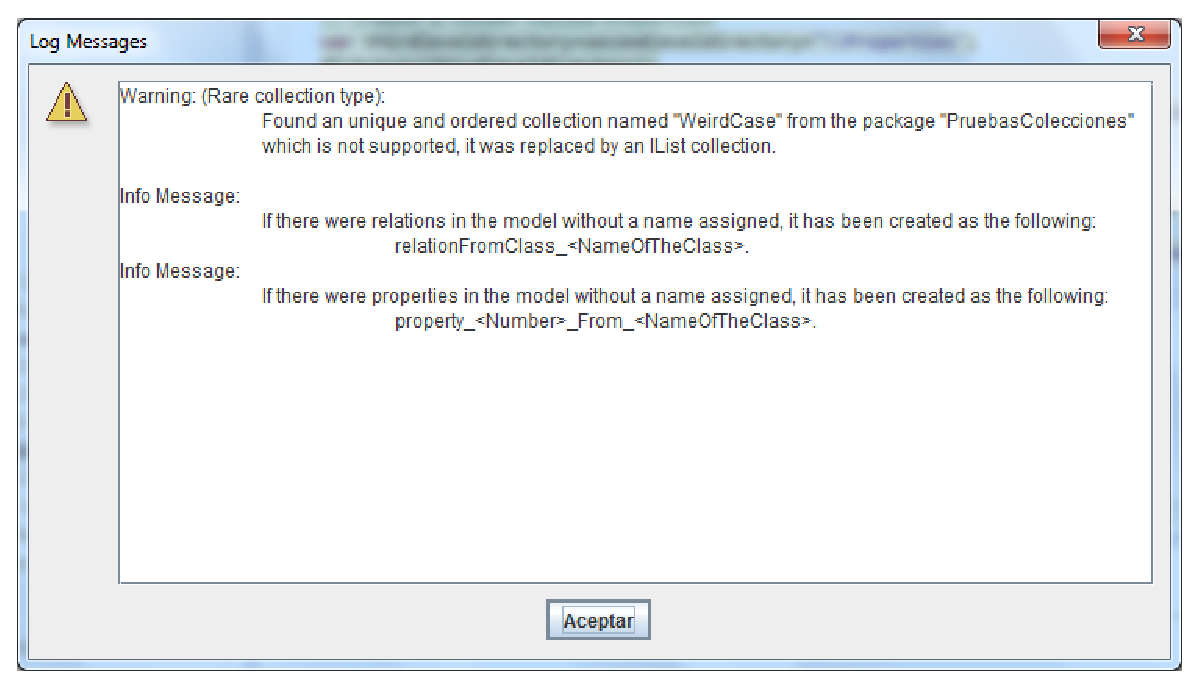
\includegraphics[width=.75\linewidth]{domainEngineering/images/FinalWindow.eps} \\
  \caption{Log mostrado al finalizar el proceso}
  \label{dom:fig:final}
\end{figure}


Las Figuras~\ref{} y~\ref{dom:fig:final} muestra dos ejemplos de estos di�logos. El primero de ellos aparecer�a al utilizar como entrada para el generador de c�digo un archivo UML que tuviese varios modelos. En este caso, el proceso de generaci�n de c�digo preguntar�a al usuario cu�l es el modelo a procesar, ya dentro de un fichero UML pueden coexistir modelos de diversa �ndole.

El segundo di�logo (Figura~\ref{dom:fig:final}) muestra, al final del proceso de generaci�n de c�digo, las incidencias que hayan podido producirse durante dicho proceso. 

La siguiente secci�n muestra, para el lector interesado, una plantilla de las descritas en esta secci�n a nivel de c�digo. 


\section{Ejemplo de Generaci�n de C�digo C\#: Caso Sencillo}
\label{domain:sec:ejsencillo}

%%==========================================================================%%
%% Author : Abascal Fern�ndez, Patricia                                     %%
%% Author : S�nchez Barreiro, Pablo                                         %%
%% Version: 1.1, 21/04/2013                                                 %%
%%                                                                          %%
%% Memoria del Proyecto Fin de Carrera                                      %%
%% Domain Engineering/Ejemplo de Generaci�n de C�digo C#: Caso Sencillo     %%
%%==========================================================================%%
\begin{figure}[tb!]
\begin{center}
\begin{footnotesize}
\begin{verbatim}
01 [%import "ReturnParameterCreation.egl";
02 import "ParametersCreation.egl";
03 import "../Operations.eol";
04 operation Element classMethods(currentPackage: String, path: String): String {   		
05  ...
06  opers=private()+void()+currentPackage+"_init"
          +self.firstToUpperCase()+" ( ) {}\n\t\t";
07  ...
08  for (oper in self.getOperations()){
09      for (par in oper.ownedParameter){
10          ...	
11          if (oper.type==null){
12              isReturn=false;
13          }else{
14              if (par.direction.toString().equals("return")){
15                  if (not par.type.name.isDefined()){
16                      isReturn=false;
17                  }else{
18                      isReturn=true;
19                  }//if-par-type
20              }//if-par-direction
21          }//if-oper-type
22      }//for-parameters
23      if (isReturn){
24          operations_return.add(oper);
25      }else{
26          operations_void.add(oper);
27      }		
28  }//for-operations	
29  for (oper in operations_void) {
30      if (oper.name==""){
31          methodname="method_"+iter;
32      }else{
33          methodname=oper.name;
34		}
35      opers=opers+oper.visibility()+oper.abstract()+oper.esStatic()+virtual()
              +void()+currentPackage+"_"+methodname
              +" ("+oper.parameters(currentPackage, path)+") {}\n\t\t";
36      // Increase the iterator
37      iter=iter+1;
38  }
39  for (oper in operations_return) {
40      if (oper.name==""){
41          methodname="method_"+iter;
42      }else{
43          methodname=oper.name;
44      }
45      opers=opers+oper.visibility()+oper.abstract()+oper.esStatic()+virtual()
             +oper.returnParameter(currentPackage, path)+" "+currentPackage+"_"+methodname
             +" ("+oper.parameters(currentPackage, path)+") {}\n\t\t";
46      // Increase the iterator
47      iter=iter+1;
48  }
49  return opers;
50 }%]
\end{verbatim}
\end{footnotesize}
\end{center}
\caption{Implementaci�n del generador de c�digo \imp{MethodsCreation}}
\label{dom:code:method}
\end{figure}

Para introducir al lector en la implementaci�n de los generadores de c�digo, vamos a analizar en detalle uno de los generadores de c�digo m�s sencillos: \imp{MethodsCreation}, el fichero fuente aparece en la figura \ref{dom:code:method}. Vamos a proceder al an�lisis detallado del mismo:
\begin{itemize}
  \item L�neas 1-3, generadores de c�digo que utiliza y fichero \imp{Operations.eol} que contiene las funciones b�sicas comunes a los generadores de c�digo.
  \item L�nea 4, descripci�n de la funci�n que retornar� el texto generado.
  \item L�nea 6, texto correspondiente al constructor de la clase de la forma $<$nombre del paquete$>$\_init$<$nombre de la clase$>$.
  \item L�neas 8-28, tratamos una a una todas las operaciones descritas en elemento actual (clase o interfaz).
  \item L�neas 9-22, en cada operaci�n recorremos todos y cada uno de los par�metros.
  \item L�neas 11-13, si la operaci�n no tiene definido un tipo, es decir, si el usuario ha obviado especificar si la funci�n devuelve una colecci�n, un entero, un elemento de una clase, etc, por defecto se trata como una operaci�n void (operaci�n que no retorna ning�n valor).
  \item L�nea 15, si la operaci�n tiene un tipo de retorno definido, comprobamos si dicho par�metro es de retorno.
  \item L�nea 16, si el par�metro es de retorno pero no est� definido vuelve a ser tratada como una operaci�n void.
  \item L�nea 18, si el par�metro es de retorno y tiene un tipo definido se trata de una operaci�n que s� retorna un valor.
  \item L�nea 24, si la operaci�n que est� siendo analizada retorna un valor, se a�ade a la lista de operaciones que devuelven un valor.
  \item L�nea 26, si la operaci�n que est� siendo analizada no retorna un valor, se a�ade a la lista de operaciones que no devuelven un valor.
  \item L�nea 29-38, a�adir al string resultado la informaci�n correspondiente a los m�todos de la clase actual que no retornan ning�n valor (m�todos void).
  \item L�nea 31, si el m�todo no tiene un nombre definido, se otorga un nombre por defecto.
  \item L�nea 35, se realizan llamadas a los generadores de c�digo para obtener los par�metros de la funci�n.
  \item L�nea 39-48, de manera an�loga a las operaciones que no retornan ning�n valor, se procede a a�adir al string resultado los m�todos de la clase que s� retornan un valor.
  \item L�nea 49, se retorna el string con todos los m�todos de la clase o interfaz actual.
\end{itemize}

Un vez explicado un ejemplo sencillos, las siguiente secci�n {domain:sec:ejcomplejo} explica ejemplos m�s complejos que quedan a la curiosidad del lector.



\section{Ejemplo de Generaci�n de C�digo C\#: Caso Complejo}
\label{domain:sec:ejcomplejo}

%%==========================================================================%%
%% Author : Abascal Fern�ndez, Patricia                                     %%
%% Author : S�nchez Barreiro, Pablo                                         %%
%% Version: 1.2, 23/04/2013                                                 %%
%%                                                                          %%
%% Memoria del Proyecto Fin de Carrera                                      %%
%% Domain Engineering/Ejemplo de Generaci�n de C�digo C#: Caso Complejo     %%
%%==========================================================================%%
Antes de comenzar a exponer los ejemplos m�s complejo, vamos a introducir aquellos conceptos que pasamos por algo en la secci�n \ref{domain:sec:transf} dada su complejidad: las relaciones bidireccionales y la herencia m�ltiple.

 \paragraph{Relaciones Bidireccionales} \ \\
 \begin{figure}[!tb]
  \centering
  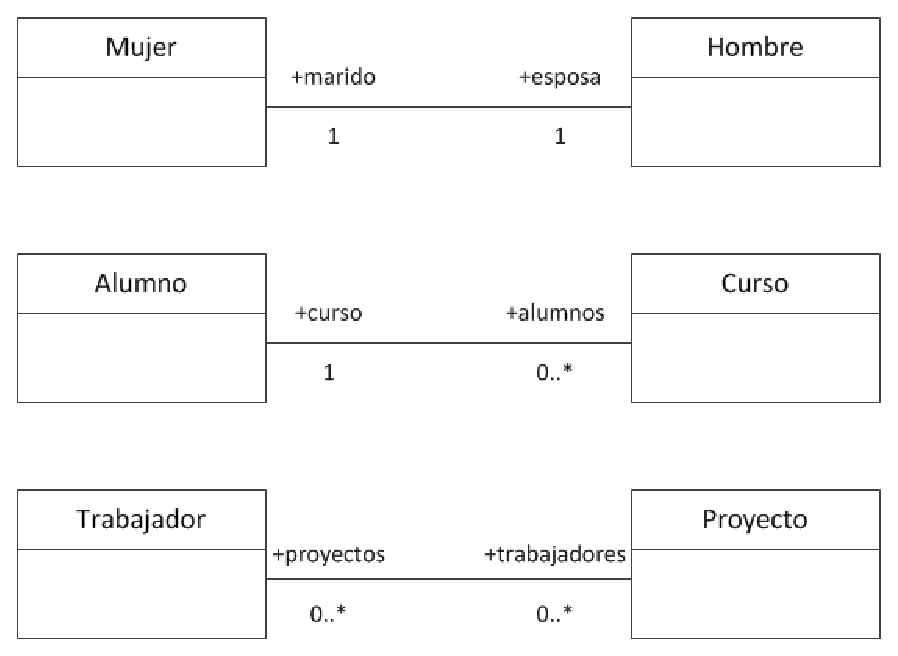
\includegraphics[width=.75\linewidth]{domainEngineering/images/bidireccionales.eps} \\
  \caption{Tipos de relaciones bidireccionales}
  \label{dom:fig:bid}
\end{figure}

Las relaciones bidireccionales son aquellas en las que ambas clases relacionadas disponen de atributos de la clase opuesta. Existen tres tipos de relaciones bidireccionales:
 \begin{itemize}
   \item \emph{Bidireccionalidad one to one}, en las que cada clase recibe un elemento de la clase opuesta (figura \ref{dom:fig:bid}, Mujer-Marido).
   \item \emph{Bidireccionalidad one to many}, en la que una de las clases recibe un elemento de la clase destino y la otra recibe una colecci�n de elementos de la clase opuesta (figura \ref{dom:fig:bid}, Alumno-Curso).
   \item \emph{Bidireccionalidad many to many}, en la que ambas clases reciben colecciones de la clase opuesta (figura \ref{dom:fig:bid}, Trabajadores-Proyectos).
 \end{itemize}

 Llegados a este punto, bas�ndonos en los ejemplos de la figura \ref{dom:fig:bid} nos surgen algunas preguntas:
 \begin{enumerate}
   \item �Si una mujer A tiene un esposo B y ese esposo B tiene una mujer que no sea A?
   \item �Si un alumno tiene asignado un curso pero ese curso no tiene a dicho alumno en su lista de alumnado?
   \item �Si un trabajador tiene asignado un proyecto pero en el listado de trabajadores dicho trabajador no aparece?
 \end{enumerate}
�Existe alguna forma de poner soluci�n a estos problemas?, la respuesta es s�, a la hora de tratar este tipo de relaciones bidireccionales en los generadores de c�digo correspondientes no basta con generar las propiedades tal como hemos estado haciendo hasta ahora sino que debemos implementar las propiedades a generar de una forma cuidadosa y exhaustiva para que no se produzcan este tipo de incoherencias, incluso recurriendo a la creaci�n de m�todos adicionales. Veamos a grandes rasgos en la tabla \ref{dom:table:bid} c�mo ser�a la implementaci�n de la relaci�n bidireccional one to one:
\begin{table}%
\begin{tabularx}{15cm}{|l|X|X|}
 \hline
{}&{\textbf{Mujer soltera}}&{\textbf{Mujer casada}} \\ \hline
{\textbf{Hombre soltero}} &
                Se casan el hombre soltero y la mujer soltera.
&  La mujer casada se divorcia. El antiguo marido de la mujer divorciada queda soltero. La mujer divorciada y el hombre soltero se casan. \\ \hline
{\textbf{Hombre casado}} & El hombre casado se divorcia. La antigua mujer del marido divorciado queda soltera. Se casan la mujer soltera y el hombre divorciado.
& El hombre casado se divorcia. La antigua mujer del marido divorciado queda soltera. La mujer casada se divorcia. El antiguo marido de la mujer divorciada queda soltero. Se casan la mujer divorciada y el hombre divorciado. \\ \hline
\end{tabularx}
\caption{Soluci�n para evitar incoherencias en el c�digo C\# en la bidireccionalidad one to one}
\label{dom:table:bid}
\end{table}%
El siguiente paso ser�a pasar dicha tabla a c�digo C\# y comprobar que funciona correctamente. Se sigue un proceso an�logo para el resto de relaciones bidireccionales.

\paragraph{Herencia m�ltiple} \ \\

\begin{figure}[!tb]
  \centering
  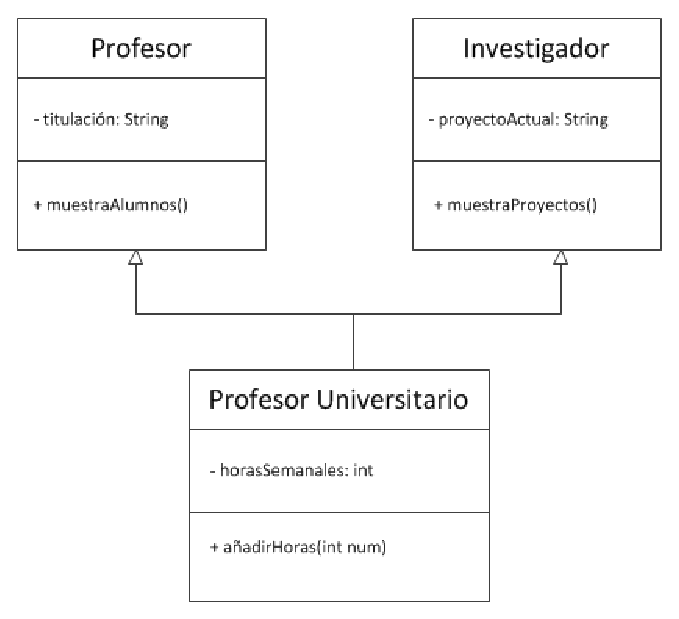
\includegraphics[width=.50\linewidth]{domainEngineering/images/herenciamultiple.eps} \\
  \caption{Tipos de relaciones bidireccionales}
  \label{dom:fig:her}
\end{figure}



\section{Sumario}
